\documentclass[12pt,a4paper]{article}
\usepackage[utf8]{inputenc}
\usepackage[russian]{babel}
\usepackage{amsmath}
\usepackage{amsfonts}
\usepackage{amssymb}
\usepackage{graphics}
\usepackage{placeins}
\usepackage[pdftex]{graphicx}
\usepackage{lscape}
\usepackage{listings}
\author{Анастасия Тарасова}
\title{Отчет по лабораторной работе №2 :\\ Утилита для исследования сети и сканер портов Nmap, Инструмент тестов на проникновение Metasploit}
\begin{document}
\maketitle
\section{Утилита для исследования сети и сканер портов Nmap}
\subsection{Цель работы}
Изчение \textbf{nmap} - свободной утилиты, предназначенной для разнообразного настраиваемого сканирования IP-сетей с любым количеством объектов, определения состояния объектов сканируемой сети (портов и соответствующих им служб).
\subsection{Ход работы}
Определить набор и версии сервисов запущенных на компьютере в диапазоне адресов.

\subsubsection{Поиск активных хостов}

\verb+db_nmap -sN 100.0.0/24+ - поиск активных хостов\\

\textbf{Вывод:}

\begin{lstlisting}
Starting Nmap 6.47 ( http://nmap.org ) at 2015-03-29 18:01 EDT
Nmap scan report for 100.0.0.24
Host is up (0.00020s latency).
Not shown: 977 closed ports
PORT     STATE         SERVICE
21/tcp   open|filtered ftp
22/tcp   open|filtered ssh
23/tcp   open|filtered telnet
25/tcp   open|filtered smtp
53/tcp   open|filtered domain
80/tcp   open|filtered http
111/tcp  open|filtered rpcbind
139/tcp  open|filtered netbios-ssn
445/tcp  open|filtered microsoft-ds
512/tcp  open|filtered exec
513/tcp  open|filtered login
514/tcp  open|filtered shell
1099/tcp open|filtered rmiregistry
1524/tcp open|filtered ingreslock
2049/tcp open|filtered nfs
2121/tcp open|filtered ccproxy-ftp
3306/tcp open|filtered mysql
5432/tcp open|filtered postgresql
5900/tcp open|filtered vnc
6000/tcp open|filtered X11
6667/tcp open|filtered irc
8009/tcp open|filtered ajp13
8180/tcp open|filtered unknown
MAC Address: 08:00:27:D4:D7:99 (Cadmus Computer Systems)

Nmap scan report for 100.0.0.23
Host is up (0.0000050s latency).
All 1000 scanned ports on 100.0.0.23 are closed

Nmap done: 256 IP addresses (2 hosts up) scanned in 31.31 seconds

\end{lstlisting}
\newpage
\subsubsection{Определить открытые порты}

\verb+db_nmap -sS 100.0.0/24+ - просмотр активных портов\\

\textbf{Вывод:}

\begin{lstlisting}
Starting Nmap 6.47 ( http://nmap.org ) at 2015-03-29 18:33 EDT
Nmap scan report for 100.0.0.24
Host is up (0.00011s latency).
Not shown: 977 closed ports
PORT     STATE SERVICE
21/tcp   open  ftp
22/tcp   open  ssh
23/tcp   open  telnet
25/tcp   open  smtp
53/tcp   open  domain
80/tcp   open  http
111/tcp  open  rpcbind
139/tcp  open  netbios-ssn
445/tcp  open  microsoft-ds
512/tcp  open  exec
513/tcp  open  login
514/tcp  open  shell
1099/tcp open  rmiregistry
1524/tcp open  ingreslock
2049/tcp open  nfs
2121/tcp open  ccproxy-ftp
3306/tcp open  mysql
5432/tcp open  postgresql
5900/tcp open  vnc
6000/tcp open  X11
6667/tcp open  irc
8009/tcp open  ajp13
8180/tcp open  unknown
MAC Address: 08:00:27:D4:D7:99 (Cadmus Computer Systems)

Nmap scan report for 100.0.0.23
Host is up (0.0000050s latency).
All 1000 scanned ports on 100.0.0.23 are closed

Nmap done: 256 IP addresses (2 hosts up) scanned in 29.82 seconds
\end{lstlisting}
\newpage
\subsubsection{Определить версии сервисов}
\verb+db_nmap -sV 100.0.0/24+ - показать версии сервисов\\

\textbf{Вывод:}

\begin{lstlisting}
Starting Nmap 6.47 ( http://nmap.org ) at 2015-03-29 18:51 EDT
Nmap scan report for 100.0.0.24
Host is up (0.00015s latency).
Not shown: 977 closed ports
PORT     STATE SERVICE     VERSION
21/tcp   open  ftp         vsftpd 2.3.4
22/tcp   open  ssh         OpenSSH 4.7p1 Debian 8ubuntu1
(protocol 2.0)
23/tcp   open  telnet      Linux telnetd
25/tcp   open  smtp        Postfix smtpd
53/tcp   open  domain      ISC BIND 9.4.2
80/tcp   open  http        Apache httpd 2.2.8 ((Ubuntu) DAV/2)
111/tcp  open  rpcbind     2 (RPC #100000)
139/tcp  open  netbios-ssn Samba smbd 3.X (workgroup: WORKGROUP)
445/tcp  open  netbios-ssn Samba smbd 3.X (workgroup: WORKGROUP)
512/tcp  open  exec        netkit-rsh rexecd
513/tcp  open  login?
514/tcp  open  shell?
1099/tcp open  rmiregistry GNU Classpath grmiregistry
1524/tcp open  shell       Metasploitable root shell
2049/tcp open  nfs         2-4 (RPC #100003)
2121/tcp open  ftp         ProFTPD 1.3.1
3306/tcp open  mysql       MySQL 5.0.51a-3ubuntu5
5432/tcp open  postgresql  PostgreSQL DB 8.3.0 - 8.3.7
5900/tcp open  vnc         VNC (protocol 3.3)
6000/tcp open  X11         (access denied)
6667/tcp open  irc         Unreal ircd
8009/tcp open  ajp13       Apache Jserv (Protocol v1.3)
8180/tcp open  http        Apache Tomcat/Coyote JSP engine 1.1
1 service unrecognized despite returning data. If you know the
service/version, please submit the following fingerprint at
http://www.insecure.org/cgi-bin/servicefp-submit.cgi :
SF-Port514-TCP:V=6.47%I=7%D=3/29%Time=551881FD%P=i686-pc-linux-
gnu%r(NULL,
SF:33,"\x01getnameinfo:\x20Temporary\x20failure\x20in\x20name
\x20resolutio
SF:n\n");
MAC Address: 08:00:27:D4:D7:99 (Cadmus Computer Systems)
Service Info: Hosts:  metasploitable.localdomain, localhost,
irc.Metasploitable.LAN; OSs: Unix, Linux; CPE: cpe:/o:linux:
linux_kernel

Nmap scan report for 100.0.0.23
Host is up (0.0000050s latency).
All 1000 scanned ports on 100.0.0.23 are closed

Service detection performed. Please report any incorrect results
at http://nmap.org/submit/ .
Nmap done: 256 IP addresses (2 hosts up) scanned in 39.96 seconds
\end{lstlisting}
\newpage
\subsubsection{Изучить файлы nmap-services, nmap-os-db, nmap-service-probes}

\textbf{nmap-service-probes}

По аналогии с подсистемой определения ОС, Nmap использует
простой текстовый файл для хранения тестов и сигнатур подсисте-
мы определения версий. Файл этот называется nmap-service-probes.
Как принято в файлах ОС UNIX, nmap-service-probes состоит из
строк. Строки, начинающиеся с символа «hash» воспринимаются
как комментарии и игнорируются обработчиком. Пустые строки
также не обрабатываются. Строки, подлежащие обработке, долж-
ны содержать следующие директивы:
\begin{itemize}
\item Probe <protocol> <probename> <probesendstring>

Директива «probe» (тест) указывает Nmap, какие данные отправ-
лять в процессе определения служб. Аргументы этой директивы
11следующие:
\begin{itemize}
\item Protocol – тип протокола. Может быть указан один из протоко-
лов TCP или UDP. Nmap будет использовать только те тесты, тип
протокола которых совпадает с рабочтм протоколом проверяемой
службы.
\item Probename – название теста. Используется в отпечатке службы для
указания, на какой тест был получен ответ. Название может быть
произвольным (удобным для пользователя).
\item Probestring – строка, используемая для тестового запроса. Долж-
на начинаться и заканчиваться символом-ограничителем «q». Меж-
ду ограничителями находится непосредственно сама строка, пере-
даваемая в качестве теста.
\end{itemize}
\item match <service> <pattern> [versioninfo]

Директива «match» указывает Nmap на то, как точно определить
службу, используя полученный ответ на запрос, отправленный преды-
дущей директивой. Эта директива используется в случае, когда по-
лученный ответ полностью совпадает с шаблоном. При этом тести-
рование порта считается законченным, а при помощи дополнитель-
ных спецификаторов Nmap строит отчет о названии приложения,
номере версии и дополнительной информации, полученной в ходе
проверки. Директива имеет следующие аргументы:
\begin{itemize}
\item Service – название службы, для которой приведен шаблон. Напри-
мер, ssh, smtp, http, или SNMP.
\item Pattern – шаблон, с которым должен совпадать полученный ответ.
Формат шаблона аналогичен принятому в языке Perl, и имеет сле-
дующий синтаксис: «m/[regex]/[opts]». Литерал «m» указывает на
начало строки. Прямой слэш (’/’) является разделителем, вместо
которого может быть подставлен любой печатаемый символ (при
этом вместо второго слэша должен быть подставлен такой же сим-
вол). Regex – это регулярное выражение, принятое в языке Perl. В
настоящее время поддерживаются только две опции – это ’i’ (сни-
мает чувствительность выражения к регистру) и ’s’, включающая
12символ перевода строки в спецификаторе типа ’.’ .
\item Versioninfo – это поле имеет следующий формат: v/vendorproductname/version/info/,
где слэш может быть заменен любым разделителем. Любое из трех
полей может быть пустым. Кроме этого, поле само может быть пу-
стым, и это означает, что дополнительная информация о службе
отсутствует. Поле vendorproductname содержит название произво-
дителя и имя службы, например, «SunSolaris rexecd», «ISC Bind
named», или «Apache httpd». Поле version содержит «номер» вер-
сии (в кавычках потому, что может обозначаться не числовым зна-
чением, а напротив, состоять из нескольких слов). Поле info содер-
жит дополнительную полезную информацию, которая может при-
годиться на этапе сканирования (например, номер протокола сер-
вера ssh).
\end{itemize}
\item softmatch <service> <pattern>

Директива softmatch имеет формат, аналогичный директиве match.
Основное отличие заключается в том, что после совпадения приня-
того ответа с одним из шаблонов softmatch, тестирование будет про-
должено с использованием только тех тестов, которые относятся к
определенной шаблоном службе. Тестирование порта будет идти до
тех пор, пока не будет найдено строгое соответствие («match») или
не закончатся все тесты для данной службы. Аргументы те же са-
мые, только, конечно, отсутствует versioninfo.

\item ports <portlist>

Эта директива группирует порты, которые обычно закрепляются
за идентифицируемой данным тестом службой. Синтаксис пред-
ставляет собой упрощенный формат опции ‘-p’.

\item sslports <portlist>

Аналогично описанной выше, эта директива указывает порты, обыч-
но используемые совместно с SSL. Например, в тесте HTTP объяв-
лено ’sslports 443’, а в тесте SMTP есть строка ’sslports 465’.

\item totalwaitms <milliseconds>

Редко используемая директива. Она указывает, сколько времени (в
миллисекундах) необходимо ждать ответ, прежде чем прекратить
тест службы.
\end{itemize}

\textbf{nmap-services}

Nmap, как известно, умеет делать много полезных вещей: это и
определение операционной системы при помощи снятия отпечатков
стека TCP/IP, многофункциональный ping-опрос, вычисление вре-
менных параметров, сканирование протоколов и т.д. Однако исто-
рическое его предназначение – это, конечно, сканирование портов.
Укажите Nmap’у интересующий Вас хост – и он может сообщить
Вам, что порты 25/tcp, 80/tcp и 35/udp хоста открыты. Используя
собственную базу данных, размещенную в файле nmap-services и
содержащую свыше 2200 названий «общеизвестных» служб, напро-
тив каждого номера обнаруженного порта Nmap укажет возмож-
ное назначение этого порта: относится ли он к почтовому серверу
(SMTP), веб-серверу (HTTP) или к службе DNS. При этом резуль-
тат определения службы, закрепленной за «общеизвестным» пор-
том, практически всегда совпадает с действительностью, поскольку
все почтовые сервера, например, должны «сидеть» на 25-м порту.
Но не стоит забывать о том, что люди могут и ЗАПУСКАЮТ служ-
бы, закрепляя их за весьма необычными портами.

\textbf{nmap-os-db}

Одна из наиболее известных функциональных возможностей Nmap
это удаленное определение ОС на основе анализа работы стека
TCP/IP. Nmap посылает серию TCP и UDP пакетов на удаленный
хост и изучает практически каждый бит в ответах. После проведе-
ния дюжины тестов таких как TCP ISN выборки, поддержки оп-
ций TCP, IP ID выборки, и анализа продолжительности процедуры
инициализации, Nmap сравнивает результаты со своей nmap-os-db
базой данных, состоящей из более чем тысячи известных наборов
типичных результатов для различных ОС и, при нахождении со-
ответствий, выводит информацию об ОС. Каждый набор содер-
жит свободное текстовое описание ОС и классификацию, в которой
14указаны название производителя (напр. Sun), название ОС (напр.
Solaris), поколение ОС (напр. 10), и тип устройства (). OS, and a
classification which provides the vendor name (e.g. Sun), underlying
OS (e.g. Solaris), OS generation (e.g. 10), and device type (для общих
целей, роутер, коммутатор (switch), игровая консоль и т.д.).
\subsubsection{Добавить новую сигнатуру службы в файл nmap-service-probes}
Запущен сервер. Его исходные файлы находятся в папке \verb+Programming\MinimalTCPServer+


Далее установлен тип подключения Kali linux  - сетевой мост. 


\verb+telnet 10.200.38.134 9090+  - проверка соединения
\begin{lstlisting}
Trying 10.200.38.134...
Connected to 10.200.38.134.
Escape character is '^]'.
Hello!!!
\end{lstlisting}
Вывод: соединение есть.

Результат работы на сервере:
\begin{lstlisting}
Client connected [100.0.0.22]...

...disconnected
Client connected [100.0.0.22]...
\end{lstlisting}
\verb+match MyService m/Hello!!!/+ - добавляем сигнатуру в файл nmap-service-probes

\verb+nmap -sS 10.200.38.134+ - просмотр активных портов и служб

\textbf{Вывод:}
\begin{lstlisting}
Starting Nmap 6.47 ( http://nmap.org ) at 2015-04-26 19:19 EDT
Nmap scan report for 10.200.38.134
Host is up (0.00068s latency).
Not shown: 997 filtered ports
PORT     STATE SERVICE
2869/tcp open  icslap
3306/tcp open  mysql
9090/tcp open  zeus-admin
MAC Address: EA:9A:8F:71:FA:E2 (Unknown)

Nmap done: 1 IP address (1 host up) scanned in 17.56 seconds

\end{lstlisting}
Как видно из листинга мы имеем открытый порт 9090, сервис zeus-admin.

\verb+nmap -sS 10.200.38.134+ - определение службы
\textbf{Вывод:}
\begin{lstlisting}
Starting Nmap 6.47 ( http://nmap.org ) at 2015-04-26 19:26 EDT
Nmap scan report for 10.200.38.134
Host is up (0.00082s latency).
Not shown: 997 filtered ports
PORT     STATE SERVICE   VERSION
2869/tcp open  http      Microsoft HTTPAPI httpd 2.0 (SSDP/UPnP)
3306/tcp open  mysql     MySQL (unauthorized)
9090/tcp open  MyService
MAC Address: EA:9A:8F:71:FA:E2 (Unknown)
Service Info: OS: Windows; CPE: cpe:/o:microsoft:windows

Service detection performed. Please report any incorrect results at http://nmap.org/submit/ .
Nmap done: 1 IP address (1 host up) scanned in 39.82 seconds

\end{lstlisting}
Видим, что имеется открытый порт 9090, сервис - MyService.
\subsubsection{Сохранить вывод утилиты в формате xml}
\verb+nmap -sV 10.200.38.134 >output.xml+\\
\verb+nmap 10.200.38.134 > output1.xml+\\
Файлы output.xml и output1.xml хранятся в той же папке что и отчет.

\subsubsection{Исследовать различные этапы и режимы работы nmap с использованием утилиты Wireshark}
Wireshark - программа для анализа сетевых протоколов, которая широко используется для захвата сетевых пакетов. Программа распространяется бесплатно. 

При переходе в Capture->Options увидим окно настройки программы, в поле интерфейс которого выбран адаптер eth0. Через него будет происходить захват пакетов.

\FloatBarrier
\begin{figure}[h!]
\centering
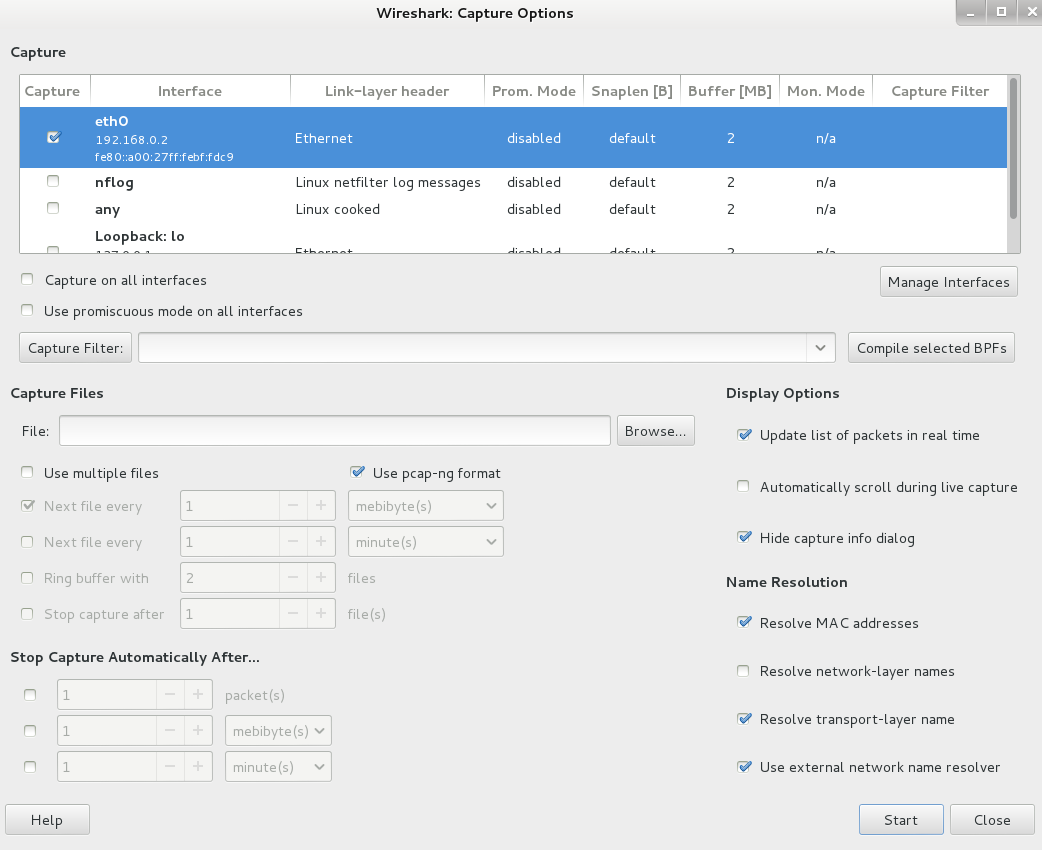
\includegraphics[scale=0.5]{res/wireshark}
\caption{Capture Options}
\end{figure}
\FloatBarrier
Запускаем Wireshark и сканируем виртуальную машину Metasploitable2.
\verb+ nmap -sV -p 2049 192.168.0.1+

Сделаем фильрацию захваченных пакетов по двум определенным IP адресам:

\verb+ip.addr==192.168.0.1 and ip.addr==192.168.0.2+
\FloatBarrier
\begin{figure}[h!]
\centering
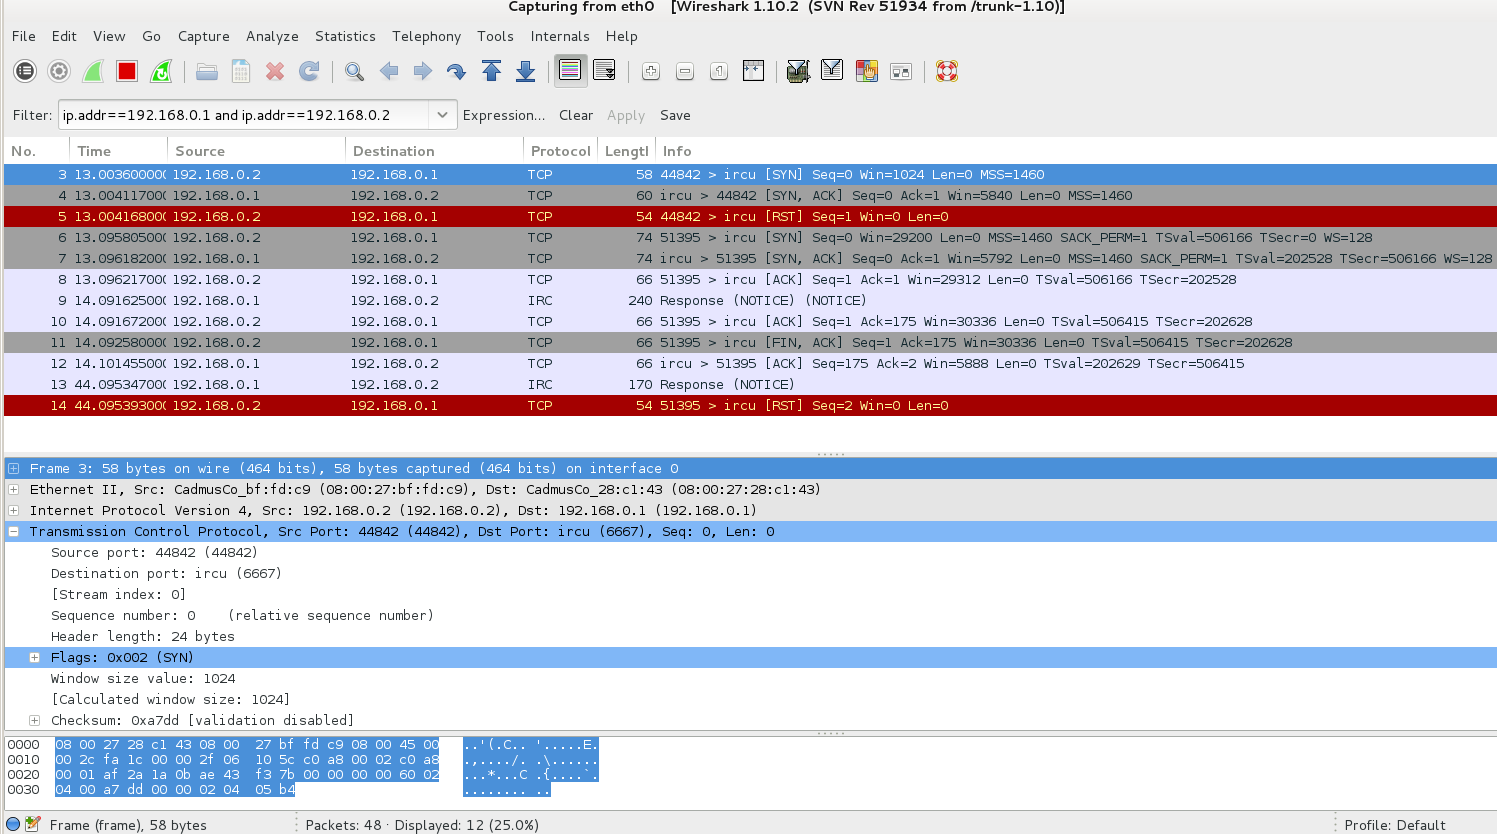
\includegraphics[scale=0.3]{res/scan1}
\caption{Фильтрация захваченных пакетов по двум определенным IP-адресам. Определение сервиса на открытый порт 6667 }
\end{figure}
\FloatBarrier
Отправляем SYN пакет, порт открыт, получаем SYN,ACK пакет, затем отправляем RST. Это значит что сканируемый порт открыт.
\FloatBarrier
\begin{figure}[h!]
\centering
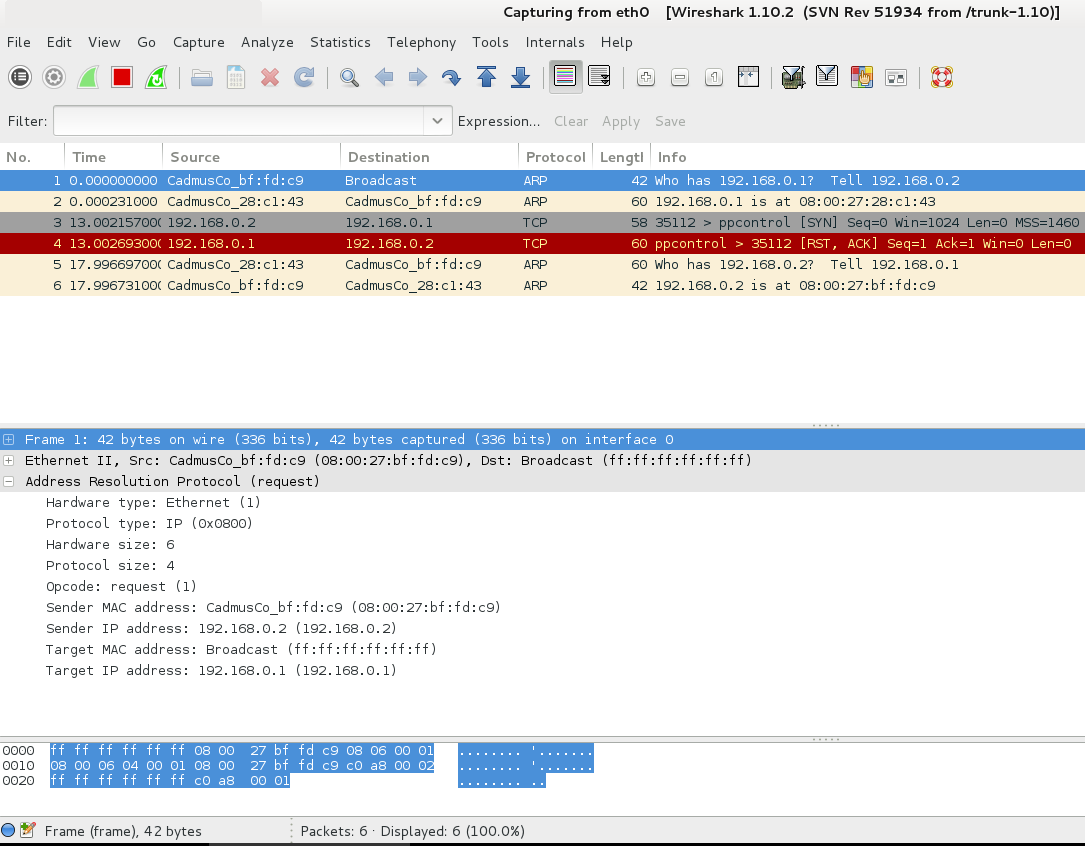
\includegraphics[scale=0.38]{res/scan2}
\caption{Фильтрация захваченных пакетов по двум определенным IP-адресам. Определение сервиса на закрытый порт 2505 }
\end{figure}
\FloatBarrier
Отправляем SYN пакет, порт открыт, получаем RST. Это значит что порт закрыт.
Это 
\verb+из состава metasploit-framework. Выбрать пять записей из файла+

\verb+nmap-service-probes и описать их работу Выбрать один скрипт из +

\verb+состава Nmap и описать его работу+
\subsection{Выводы}
Для поиска активных хостов испольховался ключ \textbf{-sN}, \textbf{--sS}
\section{Инструмент тестов на проникновение Metasploit}
\subsection{Ход работы}
\end{document} 